\section{Phương pháp}



\subsection{Mục tiêu baseline}
Phần baseline được xây dựng nhằm thiết lập một mốc tham chiếu hiệu năng cho bài toán phân vùng đa lớp thực phẩm trên bộ dữ liệu \texttt{FoodSeg103\_rebalanced}. BiSeNet (Bilateral Segmentation Network) được chọn vì đây là một kiến trúc lightweight kinh điển có chủ đích tách riêng đường đi của chi tiết không gian và ngữ cảnh ngữ nghĩa, từ đó phù hợp để làm mốc so sánh cho các cải tiến texture-aware trong giai đoạn sau.

Việc thiết lập baseline với BiSeNet tập trung vào ba mục tiêu:
\begin{itemize}[leftmargin=1.5em]
    \item \textbf{Thiết lập mốc hiệu năng}: tạo một điểm tham chiếu rõ ràng về độ chính xác và chi phí tính toán trên dữ liệu đã được tái cân bằng.
    \item \textbf{Kiểm tra giới hạn của mô hình nhẹ}: đánh giá xem một kiến trúc thời gian thực như BiSeNet suy giảm ra sao trên bài toán ingredient-level có ranh giới yếu và texture phức tạp.
    \item \textbf{Chuẩn hóa pipeline}: định nghĩa quy trình huấn luyện và đánh giá đồng nhất để làm cơ sở so sánh công bằng cho các mô-đun texture-aware hoặc boundary-aware ở bước tiếp theo.
\end{itemize}

\subsection{Kiến trúc chi tiết của BiSeNet baseline}
Theo đề xuất của Changqian Yu và cộng sự, BiSeNet được cấu thành từ hai thành phần chính nhằm giải quyết hai yêu cầu mâu thuẫn trong phân vùng ngữ nghĩa: bảo toàn chi tiết không gian và mở rộng trường thụ cảm \cite{bisenet}. Đây cũng chính là lý do mô hình được chọn cho nghiên cứu hiện tại: nó đủ nhẹ để đại diện cho ràng buộc triển khai, nhưng vẫn có sẵn cấu trúc cho phép phân tích phần mất mát local detail.

\begin{figure}[H]
    \centering
    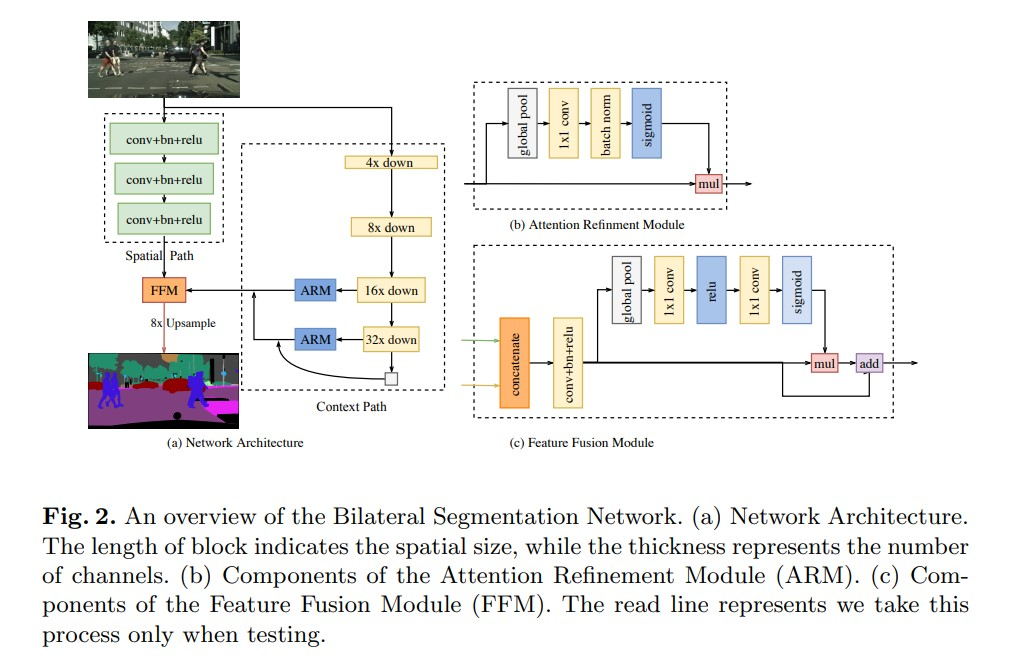
\includegraphics[width=\linewidth]{img/BiSeNET-architecture.jpg}
    \label{fig:bisenet-baseline-flow}
\end{figure}

\begin{itemize}[leftmargin=1.5em]
    \item \textbf{Spatial Path (Nhánh không gian)}: Thay vì sử dụng các phép tích chập giãn (dilated convolution) gây tốn kém tính toán, nhánh này chỉ gồm 3 tầng tích chập với stride = 2. Nhánh này trích xuất đặc trưng có kích thước bằng $1/8$ ảnh gốc, giúp bảo toàn các chi tiết cạnh và cấu trúc bề mặt của thực phẩm vốn rất dễ bị mất đi khi downsampling quá sâu.
    \item \textbf{Context Path (Nhánh ngữ cảnh)}: Nhánh này sử dụng một backbone nhẹ (như Xception hoặc ResNet18) kết hợp với Global Average Pooling (GAP) để mở rộng tối đa trường thụ cảm. Điều này giúp mạng hiểu được mối quan hệ giữa các thành phần thực phẩm trong cùng một đĩa ăn (ví dụ: cơm thường đi kèm với thức ăn mặn).
    \item \textbf{Attention Refinement Module (ARM)}: Được tích hợp vào hai giai đoạn cuối của Context Path. ARM sử dụng attention theo kênh (channel-wise attention) để tinh lọc đặc trưng, giúp mạng tập trung vào các vùng ngữ nghĩa quan trọng mà không làm tăng đáng kể chi phí tính toán.
    \item \textbf{Feature Fusion Module (FFM)}: Do đặc trưng từ Spatial Path là mức thấp (low-level) còn Context Path là mức cao (high-level), chúng không thể cộng trực tiếp. FFM thực hiện nối (concatenate) hai luồng đặc trưng, sau đó sử dụng một cấu trúc tương tự SENet để tái trọng số hóa các kênh, đảm bảo sự hòa hợp giữa chi tiết không gian và thông tin ngữ cảnh.
\end{itemize}

\subsection{Hàm mất mát và Chiến lược huấn luyện}

Mô hình được huấn luyện bằng một \emph{principal loss} tại đầu ra cuối cùng và hai \emph{auxiliary loss} gắn vào các đầu ra trung gian của Context Path theo cơ chế deep supervision. Do đó, hàm mất mát tổng được viết tường minh như sau:
\[
\mathcal{L}
=
\mathcal{L}_{p}
+ \alpha \mathcal{L}_{2}
+ \alpha \mathcal{L}_{3},
\]
trong đó $\mathcal{L}_{p}$ là loss tại đầu ra chính sau Feature Fusion Module, còn $\mathcal{L}_{2}$ và $\mathcal{L}_{3}$ lần lượt là hai loss phụ tương ứng với hai đầu ra trung gian được lấy từ Context Path. Trong BiSeNet, hệ số cân bằng được đặt là $\alpha = 1$.

Cả ba thành phần trên đều dùng \emph{pixel-wise softmax cross-entropy}. Với một đầu ra bất kỳ $o \in \{p,2,3\}$, ta có:
\[
\mathcal{L}_{o}
=
-\frac{1}{|\Omega|}
\sum_{(i,j)\in\Omega}
\log p^{(o)}_{i,j,y_{i,j}},
\]
trong đó $y_{i,j}$ là nhãn thật của pixel $(i,j)$, $\Omega$ là tập pixel hợp lệ, còn $p^{(o)}_{i,j,c}$ là xác suất softmax của lớp $c$ tại pixel $(i,j)$ ở đầu ra $o$, được tính từ logit $z^{(o)}_{i,j,c}$:
\[
p^{(o)}_{i,j,c}
=
\frac{\exp(z^{(o)}_{i,j,c})}
{\sum_{k=1}^{C}\exp(z^{(o)}_{i,j,k})}.
\]

Viết riêng từng thành phần, ta có:
\[
\mathcal{L}_{p}
=
-\frac{1}{|\Omega|}
\sum_{(i,j)\in\Omega}
\log p^{(p)}_{i,j,y_{i,j}}.
\]
\[
\mathcal{L}_{2}
=
-\frac{1}{|\Omega|}
\sum_{(i,j)\in\Omega}
\log p^{(2)}_{i,j,y_{i,j}}.
\]
\[
\mathcal{L}_{3}
=
-\frac{1}{|\Omega|}
\sum_{(i,j)\in\Omega}
\log p^{(3)}_{i,j,y_{i,j}}.
\]

Thiết kế này giúp đầu ra cuối cùng học trực tiếp mục tiêu phân đoạn, trong khi hai nhánh phụ hỗ trợ quá trình lan truyền gradient ở Context Path và làm tối ưu ổn định hơn trong giai đoạn huấn luyện. Các auxiliary loss chỉ được dùng ở pha huấn luyện; khi suy luận, mô hình chỉ sử dụng đầu ra chính.

% \subsection{Nhận xét tính phù hợp}
% Dựa trên các kết quả thực nghiệm trong paper gốc (đạt 68.4\% mIoU trên Cityscapes với tốc độ 105 FPS), BiSeNet mang lại những lợi thế lý thuyết quan trọng cho đồ án này:
% \begin{enumerate}[leftmargin=1.8em]
%     \item \textbf{Khả năng xử lý đa quy mô (Multi-scale)}: Hình ảnh thực phẩm trong tập \texttt{FoodSeg103} có sự biến thiên lớn về kích thước (một hạt ngô nhỏ so với một miếng bít tết lớn). Nhánh Context Path với GAP giúp BiSeNet bao quát được các đối tượng kích thước lớn, trong khi Spatial Path giữ được các đối tượng nhỏ.
%     \item \textbf{Hiệu quả thực thi}: So với các mô hình như DeepLabv3+ (sử dụng Atrous Spatial Pyramid Pooling phức tạp), BiSeNet đạt hiệu năng tương đương nhưng tiêu tốn ít tài nguyên tính toán hơn nhờ thiết kế song song hai nhánh đơn giản. Điều này cho phép nhóm nghiên cứu thực hiện nhiều lượt thí nghiệm (ablation study) nhanh chóng trên tập dữ liệu thực phẩm lớn.
%     \item \textbf{Tính mô-đun}: Cấu trúc ARM và FFM đủ linh hoạt để tích hợp thêm các mô-đun texture-aware, boundary-aware hoặc loss cho long-tail mà không phải thay đổi hoàn toàn khung mạng.
% \end{enumerate}
